\documentclass[11pt]{article}
\usepackage[left=2cm,top=2cm,right=2cm,bottom=2cm]{geometry}
\usepackage{graphicx}
\usepackage{setspace}
\usepackage{caption}
\usepackage{subcaption}
\usepackage{amsmath}
\usepackage{amsthm}
\usepackage[]{algorithm2e}
\usepackage{amsmath}
\usepackage[noend]{algpseudocode}
\usepackage{float}
\title{COMP 440 Homework 6}
\author{Tony Chen(xc12) and Adam Wang(sw33)}
\date{November 2016}
\begin{document}
\begin{onehalfspace}
\maketitle{}
\section{Hidden Markov Models}
\begin{itemize}
	\item
	$S = \{s_{\text{enough}},s_{\text{not}}\}$\\
	$O = \{(o_{\text{red, sleep}},o_{\text{not red, sleep}},o_{\text{red, not sleep}},o_{\text{not red, not sleep}})\}$\\
	$a_{\text{not, not}} = 0.7$\\
	$a_{\text{not, enough}} = 0.3$\\
	$a_{\text{enough, not}} = 0.2$\\
	$a_{\text{enough, enough}} = 0.8$\\
	$b_{\text{not}}(\text{red, sleep}) = 0.7\times0.3 = 0.21$\\
	$b_{\text{not}}(\text{not red, sleep}) = 0.3\times0.3 = 0.09$\\
	$b_{\text{not}}(\text{red, not sleep}) = 0.7\times0.7 = 0.49$\\
	$b_{\text{not}}(\text{not red, not sleep}) = 0.3\times0.7 = 0.21$\\
	$b_{\text{enough}}(\text{red, sleep}) = 0.2\times0.1 = 0.02$\\
	$b_{\text{enough}}(\text{not red, sleep}) = 0.8\times0.1 = 0.08$\\
	$b_{\text{enough}}(\text{red, not sleep}) = 0.2\times0.9 = 0.18$\\
	$b_{\text{enough}}(\text{not red, not sleep}) = 0.8\times0.9 = 0.72$\\
	$\pi_{\text{enough}} = 0.7$\\
	$\pi_{\text{not}} = 0.3$\\
	$\lambda = (A,B,\Pi)$ specifies the HMM model.
	\item
	$\alpha_0(\text{enough}) = 0.7$\\
	$\alpha_0(\text{not}) = 0.3$\\
	$\alpha_1(\text{enough}) = b_{\text{enough}}(\text{not red, not sleep})(\alpha_0(\text{enough})a_{\text{enough, enough}} + \alpha_0(\text{not})a_{\text{not, enough}}) = 0.468$\\
	$\alpha_1(\text{not}) = b_{\text{not}}(\text{not red, not sleep})(\alpha_0(\text{enough})a_{\text{enough, not}} + \alpha_0(\text{not})a_{\text{not, not}}) = 0.0735$\\
	\textbf{So $\mathbf{P(EnoughSleep_1|e_1) = \frac{0.468}{0.468+0.0735} = 0.8643}$.}\\
	$\alpha_2(\text{enough}) = b_{\text{enough}}(\text{red, not sleep})(\alpha_1(\text{enough})a_{\text{enough, enough}} + \alpha_1(\text{not})a_{\text{not, enough}}) = 0.071361$\\
	$\alpha_2(\text{not}) = b_{\text{not}}(\text{red, not sleep})(\alpha_1(\text{enough})a_{\text{enough, not}} + \alpha_1(\text{not})a_{\text{not, not}}) = 0.0710745$\\
	\textbf{So $\mathbf{P(EnoughSleep_2|e_1,e_2) = \frac{0.071361}{0.071361+0.0710745} = 0.5010}$.}\\
	$\alpha_3(\text{enough}) = b_{\text{enough}}(\text{red, sleep})(\alpha_2(\text{enough})a_{\text{enough, enough}} + \alpha_2(\text{not})a_{\text{not, enough}}) = 1.568\times10^{-3}$\\
	$\alpha_3(\text{not}) = b_{\text{not}}(\text{red, sleep})(\alpha_2(\text{enough})a_{\text{enough, not}} + \alpha_2(\text{not})a_{\text{not, not}}) = 13.445\times10^{-3}$\\
	\textbf{So $\mathbf{P(EnoughSleep_3|e_1,e_2,e_3) = \frac{1.568\times10^{-3}}{1.568\times10^{-3}+13.445\times10^{-3}} = 0.1044}$.}\\
	\item
	$\beta_3(\text{enough}) = 1$\\
	$\beta_3(\text{not}) = 1$\\
	\textbf{So $\mathbf{P(EnoughSleep_3|e_1,e_2,e_3) = \frac{\beta_3(\text{enough})P(EnoughSleep_3|e_1,e_2,e_3)}{\beta_3(\text{enough})P(EnoughSleep_3|e_1,e_2,e_3)+\beta_3(\text{not})(1-P(EnoughSleep_3|e_1,e_2,e_3))}}$}\\$\mathbf{=0.1044}$.\\
	$\beta_2(\text{enough}) = a_{\text{enough, not}}b_{\text{not}}(\text{red, sleep})\beta_3(\text{not})+a_{\text{enough, enough}}b_{\text{enough}}(\text{red, sleep})\beta_3(\text{enough}) = 0.058$\\
	$\beta_2(\text{not}) = a_{\text{not, not}}b_{\text{not}}(\text{red, sleep})\beta_3(\text{not})+a_{\text{not, enough}}b_{\text{enough}}(\text{red, sleep})\beta_3(\text{enough}) = 0.153$\\
	\textbf{So $\mathbf{P(EnoughSleep_2|e_1,e_2,e_3) = \frac{\beta_2(\text{enough})P(EnoughSleep_2|e_1,e_2)}{\beta_2(\text{enough})P(EnoughSleep_2|e_1,e_2)+\beta_2(\text{not})(1-P(EnoughSleep_2|e_1,e_2))}=0.2757}$.}\\
	$\beta_1(\text{enough}) = a_{\text{enough, not}}b_{\text{not}}(\text{red, not sleep})\beta_2(\text{not})+a_{\text{enough, enough}}b_{\text{enough}}(\text{red, not sleep})\beta_2(\text{enough}) = 0.023346$\\
	$\beta_1(\text{not}) = a_{\text{not, not}}b_{\text{not}}(\text{red, not sleep})\beta_2(\text{not})+a_{\text{not, enough}}b_{\text{enough}}(\text{red, not sleep})\beta_2(\text{enough}) = 0.055611$\\
	\textbf{So $\mathbf{P(EnoughSleep_1|e_1,e_2,e_3) = \frac{\beta_1(\text{enough})P(EnoughSleep_1|e_1)}{\beta_1(\text{enough})P(EnoughSleep_1|e_1)+\beta_1(\text{not})(1-P(EnoughSleep_1|e_1))}=0.7278}$.}\\
	\item
	The smoothed probabilities for $t=1,2$ are lower than the filtered probability, because smoothing takes into account the future evidence that favors the occurrence of not getting enough sleep. It is as expected that the two probabilities are the same when $t=3$.
\end{itemize}

\section{Understanding human emotions}
\begin{itemize}
\item
The hidden variable is $E_t$, whose domain is $S=\{s_{\text{sadness}},s_{\text{surprise}},s_{\text{joy}},s_{\text{disgust}},s_{\text{anger}},s_{\text{fear}}\}$\\
The observed variable is $C_t$, whose domain is $O=\{o_{\text{angular}},o_{\text{glideup}},o_{\text{descending}},o_{\text{flat}},o_{\text{irregular}}\}$
The dimensions of the state transition conditional probability table $A$ is $6\time6$.\\
The dimensions of the emission conditional probability table $B$ is $5\times6$.\\
A reasonable probability distribution $\Pi$ for $E_t$ at $t=0$ would be all six $\pi=\frac{1}{6}$.
\item
\begin{eqnarray*}
P(C_1=o_1,...,C_n=o_n) &=& \sum_{s \in S^n}P(E_1=s_1,...,E_n=s_n,C_1=o_1,...,C_n=o_n)\\
    &=& \sum_{s \in S^n}[\pi_{s_1}b_{s_1}(c_1)\prod_{i=2}^na_{s_{i-1},s_i}b_{s_i}(c_i)]
\end{eqnarray*}
\item
$P(R=x|C=c)=\alpha P(C=c)P(R=x)=\alpha \Theta_x\phi_x$
\end{itemize}

\section{Conditional random fields and named entity recognition}
\subsection*{Problem 3.3: Handling long-range dependencies}
\subsubsection*{Gibbs sampling for linear chain CRF}
\begin{eqnarray*}
P(y_t|y_{-t},x;\theta) &=& \frac{P(y|x;\theta)}{P(y_{-t}|x;\theta)}\\
    &=& \frac{G_t(y_{t-1},y_t|x;\theta)G_{t+1}(y_t,y_{t+1}|x;\theta)}{\sum_{y'\in Y}G_t(y_{t-1},y'|x;\theta)G_{t+1}(y',y_{t+1}|x;\theta)}
\end{eqnarray*}
Special case: when $t=T$ then\\
\begin{eqnarray*}
P(y_t|y_{-t},x;\theta) &=& \frac{G_t(y_{t-1},y_t|x;\theta)}{\sum_{y'\in Y}G_t(y_{t-1},y'|x;\theta)}
\end{eqnarray*}

\section{Decision networks}
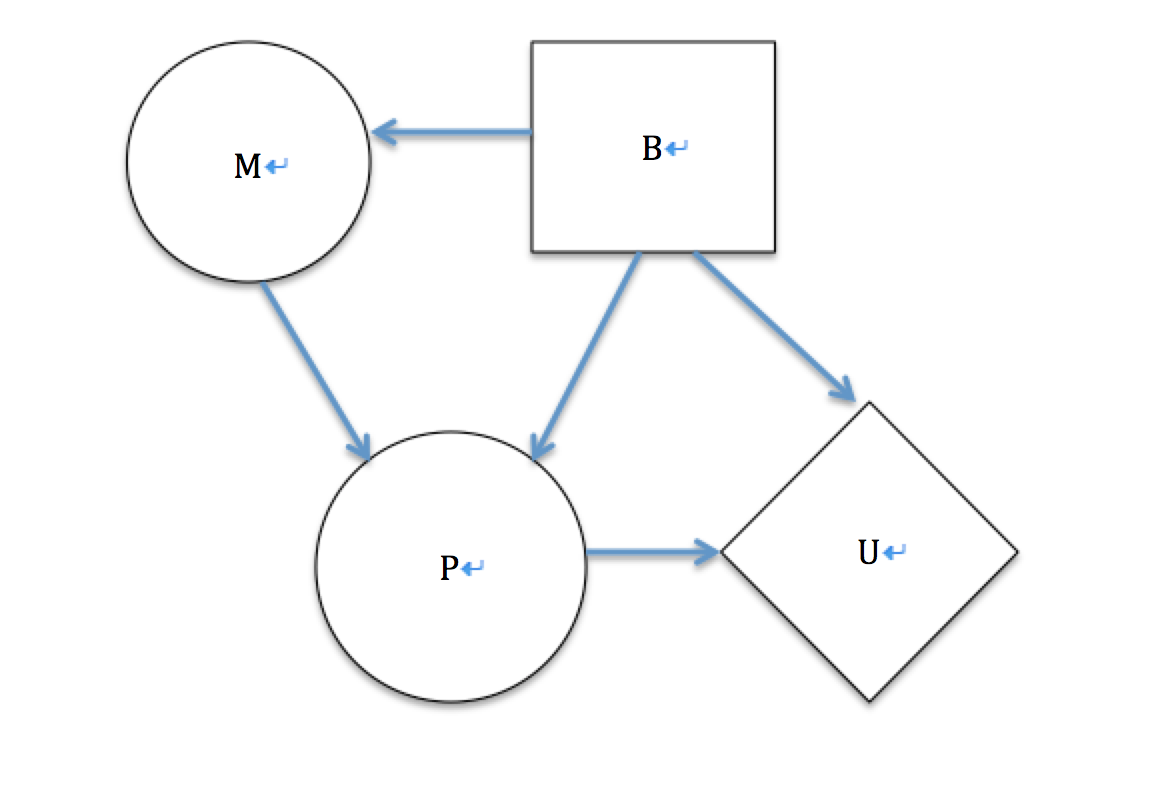
\includegraphics[width=13cm, height=9cm]{pic.png}\\
\begin{itemize}
\item
$U(b) = 2000 * P(p | b) - 100 = 2000 * (P(p | b, m) * P(m | b) + P(p | b, \neg m) * P(\neg m | b)) - 100 = 2000 * (0.9 * 0.9 + 0.5 * 0.1) - 100 = 1620$ \\
$U(\neg b) = 2000 * P(p | \neg b) = 2000 * (P(p | \neg b, m) * P(m | \neg b) + P(p | \nge b, \neg m) * P(\neg m | \neg b)) = 2000 * (0.8 * 0.7 + 0.3 * 0.3) = 1300$ \\
\item
$U(b) > U(\neg b)$, so the optimal decision for Sam is to buy the book.
\end{itemize}
\end{onehalfspace}
\end{document}